\documentclass[a4paper,11pt]{exam}
	\usepackage{graphicx}
	\usepackage[utf8]{inputenc}
	\usepackage[T1]{fontenc}
	\usepackage{listings}
	\usepackage{color}
	\usepackage{amsmath}
	\usepackage{enumerate}
	\usepackage{caption}
	\usepackage{verbatim}
	\usepackage{subcaption}
	\usepackage{tikz}
	\usepackage{graphics}
	\usepackage{txfonts}
	\usepackage{listings}
	\definecolor{dkgreen}{rgb}{0,0.5,0}
	\definecolor{gray}{rgb}{0.5,0.5,0.5}
	\definecolor{mauve}{rgb}{0.58,0,0.82}

	\lstset{frame=tb,
	  language=Python,
	  aboveskip=3mm,
	  belowskip=3mm,
	  showstringspaces=false,
	  columns=flexible,
	  basicstyle={\small\ttfamily},
	  numbers=none,
	  numberstyle=\tiny\color{gray},
	  keywordstyle=\color{blue},
	  commentstyle=\color{dkgreen},
	  stringstyle=\color{mauve},
	  breaklines=true,
	  breakatwhitespace=true
	  tabsize=3
	  }
	

\begin{document}
\begingroup 
	  \bf \Large Eletromagnetismo\\
	  \indent \normalsize André Del Bianco Giuffrida
	\endgroup
	\\ \quad
	\\
	\large{
	\emph{Lista 1 \\ Ex 7}
	\\
	\\
	Um cabo coaxial é construído usando um cilindro maciço de raio $a$, coberto concentricamente por uma superfície cilíndrica de raio $b$.\\
	O espaço entre ambos cilindros está vazio. O cilindro interno possui uma densidade de carga volumétrica $\rho$ uniforme, enquanto que o cilindro externo possui uma densidade de carga superficial uniforme $\sigma$, cujo valor garante que o conjunto completo seja eletricamente neutro.\\ 
	\\
	(a) Encontre o campo elétrico em todo o espaço: $s < a$, $a < s < b$ e $b < s$. Faça um gráfico do campo em função da posição.
	\\
	\\
	(b) Calcule a capacitância por unidade de comprimento.
	\\
	\\
	(c) Calcule a energia eletrostática por unidade de comprimento. 
	\\
	\normalsize
	\begin{center}
		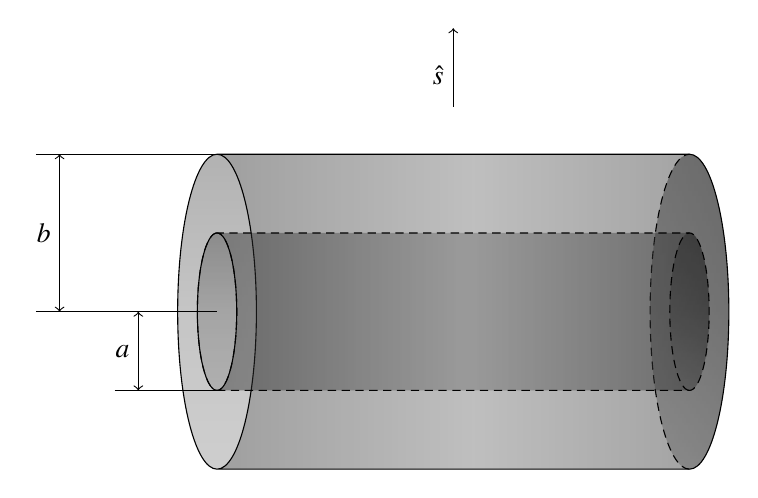
\begin{tikzpicture}
			\begin{scope}[rotate=90]
				\fill[top color=gray!50!black,bottom color=gray!10,middle color=gray,shading=axis,opacity=0.25] (0,0) circle (2cm and 0.5cm);
				\fill[left color=gray!50!black,right color=gray!50!black,middle color=gray!50,shading=axis,opacity=0.25] (2,0) -- (2,6) arc (360:180:2cm and 0.5cm) -- (-2,0) arc (180:360:2cm and 0.5cm);
				\fill[top color=gray!90!,bottom color=gray!2,middle color=gray!30,shading=axis,opacity=0.25] (0,6) circle (2cm and 0.5cm);
				\draw (-2,6) -- (-2,0) arc (180:360:2cm and 0.5cm) -- (2,6) ++ (-2,0) circle (2cm and 0.5cm);
				\draw[densely dashed] (-2,0) arc (180:0:2cm and 0.5cm);
			
				\fill[top color=gray!50!black,bottom color=gray!10,middle color=gray,shading=axis,opacity=0.25] (0,0) circle (1cm and 0.25cm);
				\fill[left color=gray!50!black,right color=gray!50!black,middle color=gray!50,shading=axis,opacity=0.25] (1,0) -- (1,6) arc (360:180:1cm and 0.25cm) -- (-1,0) arc (180:360:1cm and 0.25cm);
				\fill[top color=gray!90!,bottom color=gray!2,middle color=gray!30,shading=axis,opacity=0.25] (0,6) circle (1cm and 0.25cm);
				\draw[densely dashed] (-1,6) -- (-1,0) arc (180:360:1cm and 0.25cm) -- (1,6) ++ (-1,0) circle (1cm and 0.25cm);
				\draw[densely dashed] (-1,0) arc (180:0:1cm and 0.25cm);
				\draw (0,6) circle (1cm and 0.25cm);
			\end{scope}
				\draw (-8.3,2) -- (-6,2);
				\draw (-8.3,0) -- (-6,0);
				\draw[arrows=<->] (-8,2) -- (-8,0);
				\node at (-8.2,1) {$b$};
				\draw (-7.3,-1) -- (-6,-1);
				\draw (-7.3,0) -- (-6,0);
				\draw[arrows=<->] (-7,-1) -- (-7,0);
				\node at (-7.2,-0.5) {$a$};
				
				\draw[arrows=->] (-3,2.6) -- (-3,3.6);
				\node at (-3.2,3) {$\hat{s}$};
				
		\end{tikzpicture}
	\end{center}
	(a) \\
	\indent Calculando o Campo.
	\begin{itemize}
	\item ($s > b$) \\
		Devido ao conjunto completo ser eletricamente nulo podemos concluir que :
		\[\oint \vec{E} \cdot d\vec{a} = \int_v \frac{(\rho + \sigma)}{\epsilon_0} dv \quad \text{,} \quad (\rho + \sigma) = 0 \quad \to \quad \vec{E}(s>b) = \vec{0}\]
	\item ($s < a$)
		\[\oint \vec{E} \cdot d\vec{a} = \int_v \frac{\rho}{\epsilon_0} dv\]
		\[ \vec{E} \oint d\vec{a} = \frac{2 \pi L}{\epsilon_0} \int_0^s  s' \rho ds' \hat{s} \quad \text{,} \quad \vec{E} 2\pi L s= \frac{2 \pi L}{\epsilon_0} \int_0^s  s' \rho ds' \hat{s}\]
		
		\[\vec{E} = \frac{\rho s}{2\epsilon_0}\hat{s}\]
		
	\item ($a < s < b$)
		\[\oint \vec{E} \cdot d\vec{a} = \int_v \frac{\rho}{\epsilon_0} dv\]
		\[ \vec{E} \oint d\vec{a} = \frac{2\pi L}{\epsilon_0} \int_0^a s'\rho ds' \hat{s} \quad \text{,} \quad \vec{E} 2\pi L s = \frac{2\pi L}{\epsilon_0} \int_0^a \rho s'ds' \hat{s}\]
		\[\vec{E} = \frac{a^2 \rho}{2\epsilon_0}\frac{1}{s} \hat{s}\]

	\end{itemize}
	
	\begin{figure}[h]
		\centering
		\includegraphics[scale=0.6]{Ex.png}
		\caption{ $| \vec{E}(\vec{r}) |$ nas três regiões}
	\end{figure}
	(b)\\
	\indent Para calcular a capacitância por unidade de comprimento precisamos da diferença de potencial.
	\[C = \frac{Q}{V} \quad \text{;} \quad V(b) - V(a) = - \int_a^b \vec{E} \cdot d\vec{l}\]
	\[ V(b) - V(a) = - \int_a^b \frac{a^2 \rho}{2\epsilon_0}\frac{1}{s} ( \hat{s} \cdot d\vec{l} \, ) \]
	\[ V(b) - V(a) = -\frac{a^2 \rho}{2\epsilon_0} \int_{a}^{b} \frac{1}{s'} ds' \quad \text{,} \quad V(b) - V(a) = -\frac{a^2 \rho}{2\epsilon_0} \ln{\Bigg(\frac{b}{a}\Bigg)}  \]

	Pela definição da densidade de carga, $Q = \rho \pi a^2 L$ \\
	\indent Como queremos a capacitância por unidade de comprimento vamos escrever:
	
	\[ C_L = \frac{\rho \pi a^2}{V} \quad \text{,} \quad C_L = -\frac{\rho \pi a^2}{\frac{a^2 \rho}{2\epsilon_0} \ln{\Big(\frac{b}{a}\Big)}}\]
	\[ C_L = -\frac{2 \epsilon_0 \pi}{\ln{\Big(\frac{b}{a}\Big)}}\]
	(c)
	\\
	\indent Vamos calcular a energia Eletrostática por unidade de comprimento, sendo $u$ a densidade de energia (energia por unidade de volume)
	\[u = \frac{\epsilon_0}{2} E^2 \quad \text{integrando na área perpendicular a} \, \, \hat{z} \quad \int u \,da = \frac{\epsilon_0}{2} \int E^2 da\]
	\[u' = \frac{\epsilon_0}{2} \Bigg[ \int_{0}^{2\pi} \int_0^{\infty} E^2 s' ds' \Bigg] \quad u' = \frac{\epsilon_0}{2} \Bigg[ \int_{0}^{2\pi} d\phi \int_0^{\infty} E^2 s'ds' \Bigg] \]
	\[u' = \epsilon_0 \pi \Bigg[ \int_0^{a}\frac{\rho^2}{4\epsilon_0^2} s'^3 ds' + \int_a^{b} \frac{a^4 \rho^2}{4\epsilon_0^2}\frac{1}{s'} ds'  + \int_b^{\infty} 0 \, ds' \Bigg] \]
	\[u' = \frac{\rho^2\pi}{4\epsilon_0^2} \Bigg[ \quad	 \frac{s^4}{4}\Bigg|_{s=0}^{a} \quad +\quad  a^4\ln{(s)}\Bigg|_{s=a}^{b} \quad \Bigg]\]
	\[ u'= \frac{\rho^2\pi a^4}{4\epsilon_0^2} \Bigg[ \frac{1}{4} + \ln{\Bigg(\frac{b}{a}\Bigg)} \Bigg] \]
	de modo que $u'$ é a Energia por unidade de comprimento, ou pode-se chamar $u'$ de Densidade linear de energia no cabo
	
\end{document}
